\section{Auswertung}

Hier wurden die gemessenen Intensitäten graphisch in Abhängigkeit von den Verschiebungen dargestellt, welche sich zu Beugungsbildern ergibt.

\subsection{Einzelspalt}

\begin{figure}
  \centering
  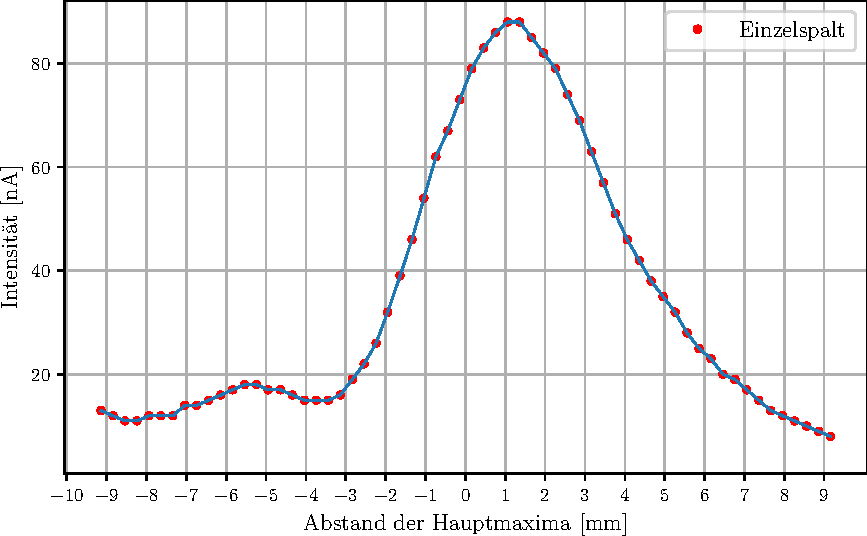
\includegraphics{content/single.pdf}
  \caption{Hier zu sehen ist die graphische Darstellung des Beugungsbildes von dem Einzelspalt.}
  \label{fig:single}
\end{figure}

Hier ist das Maximum nullter Ordnung deutlich zu sehen, und zwar bei etwa 1,2 Millimeter. Das Maximum erster Ordnung ist links schwach zu erkennen. Sie liegt bei etwa -5,5 Millimeter im Graphen. Links am Ende wird noch eine Steigung deutlich, was womöglich auf das Maximum zweiter Ordnung hinweist. Rechts hingegen ist nichts Schlüssiges.

\subsection{Doppelspalt}

\begin{figure}
  \centering
  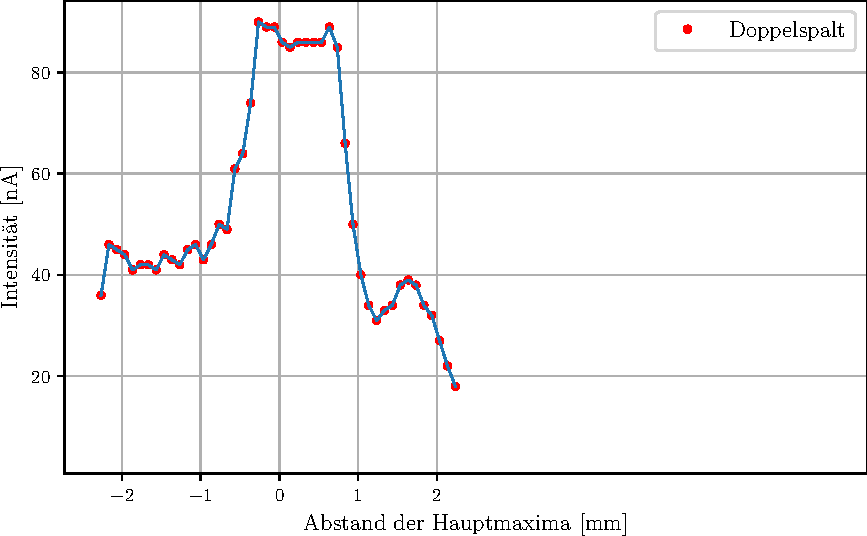
\includegraphics{content/double.pdf}
  \caption{Hier zu sehen ist die graphische Darstellung des Beugungsbildes von dem Doppelspalt.}
  \label{fig:double}
\end{figure}

Hier befindet sich das Maximum nullter Ordnung in einem Bereich zwischen -0,3 Millimeter und 0,7 Millimeter. Die Maxima erster Ordnung befinden sich bei etwa -2,3 und 1,6 Millimeter. Deutlich unter den anderen kleinen Maxima werden sie unter Betrachtung der nächsten Messpunkte, welche viel weiter unten liegen als jegliche davor.

\label{sec:Auswertung}